% hitex:master e
\documentclass[compress]{beamer}

\usepackage[english]{babel}
\usepackage[amssymb]{SIunits}

\usepackage{latexsym}
\usepackage{marvosym}

\usepackage{minted}
\usepackage{tikz}

\useoutertheme[footline=authortitle]{miniframes}
\useinnertheme{circles}
\usecolortheme{whale}
\beamertemplatenavigationsymbolsempty
\setcounter{tocdepth}{2}
%\beamerdefaultoverlayspecification{<+->}

\AtBeginSection[]{\frame{\tableofcontents[sectionstyle=show/shaded,subsectionstyle=show/show/hide]}}
%\AtBeginSection[]{\frame{\tableofcontents[currentsection]}}

% vim macros and mappings
% :let @x='0xyyu@"j'
%j6@x
%:map <F12> :wa<CR>:!hitex.pl TEMPLATE<CR><CR>
%:map <F11> :wa<CR>:!hitex.pl -a TEMPLATE<CR><CR>
%:map <F10> :!xpdf -remote latex TEMPLATE.pdf &> /dev/null &<CR><CR>
%:map <F9> :!evince TEMPLATE.pdf &> /dev/null &<CR><CR>
%:imap <F11> <Esc>:wa<CR>:!hitex.pl -a TEMPLATE<CR><CR>a
%:imap <F12> <Esc>:wa<CR>:!hitex.pl TEMPLATE<CR><CR>a


% some useful macros
\newcommand{\ignore}[1]{}
\newcommand{\lto}{\ensuremath{\leadsto}}
\newcommand{\lvsp}{\ \\[7mm]}
\newcommand{\nl}{\ \\}
\newcommand{\nvsp}{\vspace{-3ex}}
\newcommand{\see}[1]{($\to$\,\ref{#1})}
\newcommand{\svsp}{\ \\[2mm]}
\newcommand{\tab}{\rule{2em}{0pt}}
\newcommand{\todo}{\textbf{\textcolor{cyan}{TODO}}}
\newcommand{\vsp}{\ \\[5mm]}

\newenvironment{asm}{\begin{tabbing}tabs\=mnemonic\=\kill\ttfamily}{\end{tabbing}}


% function-/program-/library names and code snippets
\newcommand{\pgm}[1]{\texttt{#1}}

\newcommand{\ccr}{\pgm{CR}}
\newcommand{\clf}{\pgm{LF}}
\newcommand{\cnull}{\pgm{'\textbackslash0'}}
\newcommand{\eof}{\pgm{EOF}}
\newcommand{\gcc}{\pgm{gcc}}
\newcommand{\gdb}{\pgm{gdb}}
\newcommand{\cgets}{\pgm{gets}}
\newcommand{\libc}{\pgm{libc}}
\newcommand{\ofp}{\pgm{-fomit-frame-pointer}}
\newcommand{\readlower}{\pgm{read\_lower}}
\newcommand{\ropc}{\pgm{ropc}}
\newcommand{\ropgadget}{\pgm{ROPgadget}}
\newcommand{\system}{\pgm{system()}}

\newcommand{\add}{\pgm{add}}
\newcommand{\call}{\pgm{call}}
\newcommand{\enter}{\pgm{enter}}
\newcommand{\leave}{\pgm{leave}}
\newcommand{\mov}{\pgm{mov}}
\newcommand{\movl}{\pgm{movl}}
\newcommand{\nop}{\pgm{nop}}
\newcommand{\ret}{\pgm{ret}}
\newcommand{\sub}{\pgm{sub}}
\newcommand{\pop}{\pgm{pop}}
\newcommand{\push}{\pgm{push}}

\newcommand{\eax}{\pgm{\%eax}}
\newcommand{\ebx}{\pgm{\%ebx}}
\newcommand{\ecx}{\pgm{\%ecx}}
\newcommand{\edx}{\pgm{\%edx}}
\newcommand{\esi}{\pgm{\%esi}}
\newcommand{\edi}{\pgm{\%edi}}
\newcommand{\ebp}{\pgm{\%ebp}}
\newcommand{\esp}{\pgm{\%esp}}
\newcommand{\eip}{\pgm{\%eip}}
\newcommand{\efl}{\pgm{\%eflags}}


% other names
\newcommand{\name}[1]{\textsl{#1}}

\newcommand{\arm}{\name{ARM}}
\newcommand{\ia}{\name{IA-32}}
\newcommand{\morris}{\name{Morris worm}}
\newcommand{\ropeme}{\name{ROPEME}}
\newcommand{\ropdefender}{\name{ROPdefender}}
\newcommand{\sparc}{\name{SPARC}}
\newcommand{\sguard}{\name{StackGuard}}
\newcommand{\wx}{\name{W$\oplus$X}}
\newcommand{\xes}{\name{x86}}


% common terms
\newcommand{\att}{AT\&T}
\newcommand{\bo}{buffer overflow}
\newcommand{\canaries}{stack canaries}
\newcommand{\rtl}{return-to-\libc}
\newcommand{\ro}{return-oriented}
\newcommand{\roe}{return-oriented exploitation}
\newcommand{\rop}{return-oriented programming}
\newcommand{\shadow}{shadow stack}


\title[Return-oriented programming]{\huge{Return-oriented programming}}
\subject{IT-Security}
\author{Sebastian Neuser}
\institute{
    \Large{Seminar: IT-Security}\\[0.25cm]
    \small{University of Siegen\\
           Faculty of Science and Technology\\
           Department of Electrical Engineering and Computer Science}
}
\date{\today}

\begin{document}
    \frame{\titlepage}
    \frame{\tableofcontents[sections=1-2]}
    \frame{\tableofcontents[sections=3-5]}

    \section{Introduction}
\subsection{What is return-oriented programming?} \label{sect:what}
\frame{
    \frametitle{Buffer overflow vulnerabilities}
    simple example:
    \begin{itemize}
        \item fixed size character buffer
        \item program reads a string from the keyboard and copies it to the buffer without bounds checking
        \item number of input characters $>$ buffer size \lto\ \bo
        \item variables on the stack are overwritten -- possibly including the current function's returns address
        \item best case scenario: \pgm{SIGSEGV}
    \end{itemize}
}

\frame{
    \frametitle{Return-oriented programming}
    \begin{itemize}
        \item generalization of return-to-libc exploitation
        \item attacker uses \bo-vulnerability or something similar to inject return addresses into the stack
        \item \rtl-exploits chain together calls to library functions (\libc\ in most cases)
        \item \ro\ exploits jump a few instructions before a function's \ret\ to perform small operations
    \end{itemize}
    By carefully chaining together such jumps, an attacker can perform arbitrary computations!
}

\frame{
    \frametitle{Why care?}
    \begin{minipage}{0.9\textwidth}
    \begin{itemize}
        \item $45\%$ of recorded security vulnerabilities: possible \bo s
        \item \bo\ exploits have been used in numerous malicious software
        \item ROP: probably the most advanced \bo\ exploitation technique
        \item developed and refined over decades
    \end{itemize}
    \end{minipage}
}



\subsection{Terms and conditions} \label{sect:terms}
\frame{
    \frametitle{Terms and conditions}
    \begin{itemize}
        \item Although I don't intend to, unfortunately I tend to
              \begin{itemize}
                  \item become overzealous,
                  \item talk too fast and
                  \item speak with a slur.
              \end{itemize}
              \lto\ Please insult me, if I do!
        \item By sitting here and listening to the talk, you agree that
              \begin{itemize}
                  \item you will not use the knowledge provided here to harm anyone,
                  \item I am not responsible for anything you break while messing around with the techniques I present,
                  \item \texttt{vim} is the name of the one true editor,
                  \item proprietary software is inherently evil.
              \end{itemize}
        \item Feel free to ask questions at any time.
    \end{itemize}
}

\frame{
    \frametitle{Stack diagrams}
    \begin{itemize}
        \item Stack diagrams are depicted from the stack's top to bottom:
              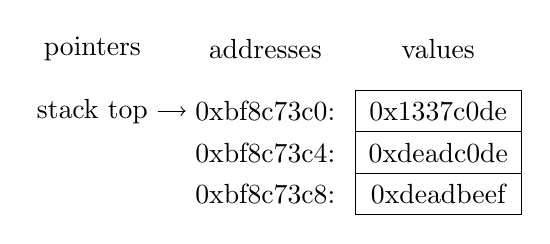
\begin{tikzpicture}
                  \tikzset{x=2.5em, y=1.5em}
                  \tikzstyle{mem}=[rectangle, draw, minimum width=6em, minimum height=1.5em]

                  \draw (0.0, 3.5)    node        (l0)    {pointers};
                  \draw (2.5, 3.5)    node        (l1)    {addresses};
                  \draw (5.0, 3.5)    node        (l2)    {values};

                  \draw (0.0, 2.0)    node        (esp0)  {stack top};
                  \draw (2.5, 2.0)    node        (a2)    {0xbf8c73c0:};
                  \draw (2.5, 1.0)    node        (a1)    {0xbf8c73c4:};
                  \draw (2.5, 0.0)    node        (a0)    {0xbf8c73c8:};
                  \draw (5.0, 2.0)    node[mem]   (s2)    {0x1337c0de};
                  \draw (5.0, 1.0)    node[mem]   (s1)    {0xdeadc0de};
                  \draw (5.0, 0.0)    node[mem]   (s0)    {0xdeadbeef};

                  \draw [->]      (esp0) -- (a2);
              \end{tikzpicture}
    \end{itemize}
}

\frame{
    \frametitle{Platform}
    Examples and demo compiled and tested with
    \begin{itemize}
        \item \texttt{gcc} version 4.7.2
        \item \texttt{gdb} version 7.4.1
        \item \unit{32}{bit} Debian GNU/Linux 7.1 \\
              \lto\ instruction set architecture: IA-32
        \item Intel Core 2 Duo P7450
    \end{itemize}
}



\subsection{Examples} \label{sect:examples}
\frame{
    \frametitle{Computer worms}
    \begin{itemize}
        \item The \morris\ aka. "Great Worm"
              \begin{itemize}
                  \item utilized a \bo-vulnerability in the \pgm{fingerd} program on Unix systems
                  \item rendered infected systems unusable within 90 minutes
              \end{itemize}
        \item The \name{Slammer} worm
              \begin{itemize}
                  \item used \bo-vulnerabilities in Microsoft's "SQL Server 2000" and "Desktop Engine 2000"
                  \item infected roughly 75000 servers in approximately 30 minutes
                  \item caused network overloads on a great scale
              \end{itemize}
        \item The \name{Sasser} worm
              \begin{itemize}
                  \item exploited a vulnerability in Microsoft's LSASS
                  \item caused systems to shut down
              \end{itemize}
    \end{itemize}
}



\subsection{History} \label{sect:history}
\frame{
    \frametitle{Timeline of \bo\ exploits}
    \begin{itemize}
        \item[1988] \morris
        \item[1996] Aleph One: "Smashing The Stack For Fun And Profit"
        \item[1997] Solar Designer: \rtl\ basics
        \item[1998] Solar Designer: security patch for the Linux kernel
        \item[2000] PaX: Implementation of \wx
        \item[2001] Nergal: function chaining with \rtl
        \item[2007] Hovav Shacham: "Return-into-libc without function calls" \\
                    \lto\ \rop
        \item[since] more and more proof, that \rop\ is a real threat
    \end{itemize}
}

    \section{Return-oriented programming in a nutshell}
\subsection{x86 crash course}
    \frame{
        \frametitle{Register set}
        \begin{description}
            \item[\eax] holds the return value of a function call.
            \item[\ebx] holds a pointer to some data.
            \item[\ecx] is used for counters in string- and loop instructions.
            \item[\edx] holds a I/O pointers.
            \item[\esi] is the source pointer in some instructions.
            \item[\edi] is the destination pointer in some instructions.
            \item[\ebp] is the stack frame- or base pointer.
            \item[\esp] is the stack pointer.
            \item[\eip] is the instruction pointer.
            \item[\efl] is the status and control register.
        \end{description}
    }

    \frame{
        \frametitle{Instruction set}
        \begin{tabular}{l|p{0.66\textwidth}}
            \mov\ \esp, \ebp    & Copies the stack pointer \esp\ to the base pointer \ebp.
            \\ \hline
            \push\ \ebp         & Updates the stack pointer \esp\ and writes the value of \ebp\ to the new top of the stack.
            \\ \hline
            \pop\ \ebp          & Reads the value at the top of the stack -- the memory location that \esp\ points to, writes it into \ebp\ and discards the value from the stack by adjusting \esp.
            \\ \hline
            \call\ func         & Pushes the return address, which is the address of the next instruction (\eip+5) onto the stack and jumps to the instruction labeled by "func:".
            \\ \hline
            \ret                & Pops the return address from the top of the stack and writes it into \eip.
        \end{tabular}
    }

    \frame{
        \frametitle{The stack}
        \begin{itemize}
            \item data section in a process' address space
            \item contains local variables and buffers
            \item arguments to function calls and the return address are also implemented using the stack
            \item \xes-family of CPUs:
                  \begin{itemize}
                      \item stack grows from higher to lower memory addresses
                      \item memory is addressed byte-wise \\
                            \lto\ \push\ increments \esp\ by 4,
                            \pop\ decrements \esp\ by 4
                  \end{itemize}
        \end{itemize}
    }

    \frame{
        \frametitle{Function calls -- \cdecl}
        \begin{itemize}
            \item parameters are \push ed to the stack in reverse order
            \item \call\ pushes the address of the next instruction onto the stack
            \item function prologue (\enter):
                  \begin{itemize}
                      \item save the base pointer \ebp
                      \item copy \esp\ to \ebp\ for \bpa
                      \item decremented \esp\ to allocate stack memory for local variables
                  \end{itemize}
            \item function epilogue (\leave):
                  \begin{itemize}
                      \item discard local variables by copying \esp\ to \ebp
                      \item restore \ebp\ by popping it from the stack
                  \end{itemize}
            \item \ret\ pops the return address off the stack and jumps to it
        \end{itemize}
    }

    \frame{
        \frametitle{Function calls -- stack diagram}
        \begin{center}
            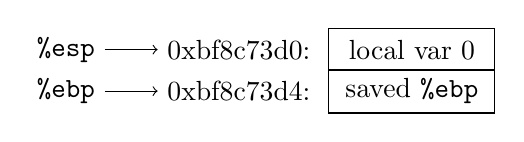
\begin{tikzpicture}
                \tikzset{x=2.5em, y=1.5em}
                \tikzstyle{mem}=[rectangle, draw, minimum width=6em, minimum height=1.5em]

                \draw (0.0, 1.0)    node        (esp)   {\esp};
                \draw (0.0, 0.0)    node        (ebp)   {\ebp};

                \draw (2.5, 1.0)    node        (a1)    {0xbf8c73d0:};
                \draw (2.5, 0.0)    node        (a0)    {0xbf8c73d4:};

                \draw (5.0, 1.0)    node[mem]   (s1)    {local var 0};
                \draw (5.0, 0.0)    node[mem]   (s0)    {saved \ebp};

                \draw [->]          (esp) -- (a1);
                \draw [->]          (ebp) -- (a0);
            \end{tikzpicture}
        \end{center}
    }

    \frame{
        \frametitle{Function calls -- stack diagram}
        \begin{center}
            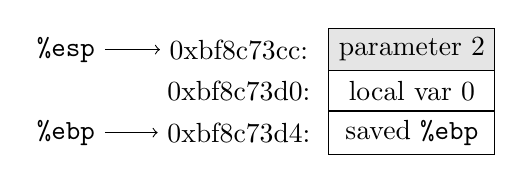
\begin{tikzpicture}
                \tikzset{x=2.5em, y=1.5em}
                \tikzstyle{mem}=[rectangle, draw, minimum width=6em, minimum height=1.5em]
                \tikzstyle{frame}=[mem, fill=black!10]

                \draw (0.0, 2.0)    node        (esp)   {\esp};
                \draw (0.0, 0.0)    node        (ebp)   {\ebp};

                \draw (2.5, 2.0)    node        (a2)    {0xbf8c73cc:};
                \draw (2.5, 1.0)    node        (a1)    {0xbf8c73d0:};
                \draw (2.5, 0.0)    node        (a0)    {0xbf8c73d4:};

                \draw (5.0, 2.0)    node[frame] (p2)    {parameter 2};
                \draw (5.0, 1.0)    node[mem]   (s1)    {local var 0};
                \draw (5.0, 0.0)    node[mem]   (s0)    {saved \ebp};

                \draw [->]          (esp) -- (a2);
                \draw [->]          (ebp) -- (a0);
            \end{tikzpicture}
        \end{center}
    }

    \frame{
        \frametitle{Function calls -- stack diagram}
        \begin{center}
            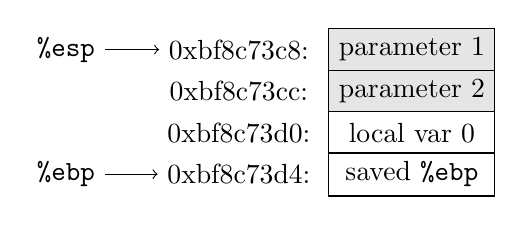
\begin{tikzpicture}
                \tikzset{x=2.5em, y=1.5em}
                \tikzstyle{mem}=[rectangle, draw, minimum width=6em, minimum height=1.5em]
                \tikzstyle{frame}=[mem, fill=black!10]

                \draw (0.0, 3.0)    node        (esp)   {\esp};
                \draw (0.0, 0.0)    node        (ebp)   {\ebp};

                \draw (2.5, 3.0)    node        (a3)    {0xbf8c73c8:};
                \draw (2.5, 2.0)    node        (a2)    {0xbf8c73cc:};
                \draw (2.5, 1.0)    node        (a1)    {0xbf8c73d0:};
                \draw (2.5, 0.0)    node        (a0)    {0xbf8c73d4:};

                \draw (5.0, 3.0)    node[frame] (p1)    {parameter 1};
                \draw (5.0, 2.0)    node[frame] (p2)    {parameter 2};
                \draw (5.0, 1.0)    node[mem]   (s1)    {local var 0};
                \draw (5.0, 0.0)    node[mem]   (s0)    {saved \ebp};

                \draw [->]          (esp) -- (a3);
                \draw [->]          (ebp) -- (a0);
            \end{tikzpicture}
        \end{center}
    }

    \frame{
        \frametitle{Function calls -- stack diagram}
        \begin{center}
            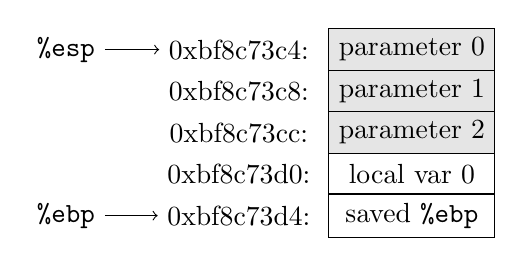
\begin{tikzpicture}
                \tikzset{x=2.5em, y=1.5em}
                \tikzstyle{mem}=[rectangle, draw, minimum width=6em, minimum height=1.5em]
                \tikzstyle{frame}=[mem, fill=black!10]

                \draw (0.0, 4.0)    node        (esp)   {\esp};
                \draw (0.0, 0.0)    node        (ebp)   {\ebp};

                \draw (2.5, 4.0)    node        (a4)    {0xbf8c73c4:};
                \draw (2.5, 3.0)    node        (a3)    {0xbf8c73c8:};
                \draw (2.5, 2.0)    node        (a2)    {0xbf8c73cc:};
                \draw (2.5, 1.0)    node        (a1)    {0xbf8c73d0:};
                \draw (2.5, 0.0)    node        (a0)    {0xbf8c73d4:};

                \draw (5.0, 4.0)    node[frame] (p0)    {parameter 0};
                \draw (5.0, 3.0)    node[frame] (p1)    {parameter 1};
                \draw (5.0, 2.0)    node[frame] (p2)    {parameter 2};
                \draw (5.0, 1.0)    node[mem]   (s1)    {local var 0};
                \draw (5.0, 0.0)    node[mem]   (s0)    {saved \ebp};

                \draw [->]          (esp) -- (a4);
                \draw [->]          (ebp) -- (a0);
            \end{tikzpicture}
        \end{center}
    }

    \frame{
        \frametitle{Function calls -- stack diagram}
        \begin{center}
            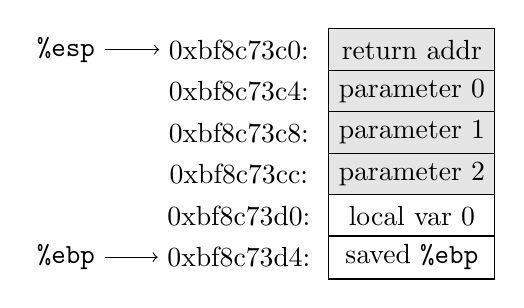
\begin{tikzpicture}
                \tikzset{x=2.5em, y=1.5em}
                \tikzstyle{mem}=[rectangle, draw, minimum width=6em, minimum height=1.5em]
                \tikzstyle{frame}=[mem, fill=black!10]

                \draw (0.0, 5.0)    node        (esp)   {\esp};
                \draw (0.0, 0.0)    node        (ebp)   {\ebp};

                \draw (2.5, 5.0)    node        (a5)    {0xbf8c73c0:};
                \draw (2.5, 4.0)    node        (a4)    {0xbf8c73c4:};
                \draw (2.5, 3.0)    node        (a3)    {0xbf8c73c8:};
                \draw (2.5, 2.0)    node        (a2)    {0xbf8c73cc:};
                \draw (2.5, 1.0)    node        (a1)    {0xbf8c73d0:};
                \draw (2.5, 0.0)    node        (a0)    {0xbf8c73d4:};

                \draw (5.0, 5.0)    node[frame] (raddr) {return addr};
                \draw (5.0, 4.0)    node[frame] (p0)    {parameter 0};
                \draw (5.0, 3.0)    node[frame] (p1)    {parameter 1};
                \draw (5.0, 2.0)    node[frame] (p2)    {parameter 2};
                \draw (5.0, 1.0)    node[mem]   (s1)    {local var 0};
                \draw (5.0, 0.0)    node[mem]   (s0)    {saved \ebp};

                \draw [->]          (esp) -- (a5);
                \draw [->]          (ebp) -- (a0);
            \end{tikzpicture}
        \end{center}
    }

    \frame{
        \frametitle{Function calls -- stack diagram}
        \begin{center}
            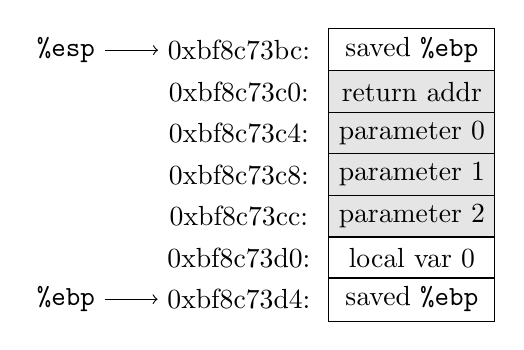
\begin{tikzpicture}
                \tikzset{x=2.5em, y=1.5em}
                \tikzstyle{mem}=[rectangle, draw, minimum width=6em, minimum height=1.5em]
                \tikzstyle{frame}=[mem, fill=black!10]

                \draw (0.0, 6.0)    node        (esp)   {\esp};
                \draw (0.0, 0.0)    node        (ebp)   {\ebp};

                \draw (2.5, 6.0)    node        (a6)    {0xbf8c73bc:};
                \draw (2.5, 5.0)    node        (a5)    {0xbf8c73c0:};
                \draw (2.5, 4.0)    node        (a4)    {0xbf8c73c4:};
                \draw (2.5, 3.0)    node        (a3)    {0xbf8c73c8:};
                \draw (2.5, 2.0)    node        (a2)    {0xbf8c73cc:};
                \draw (2.5, 1.0)    node        (a1)    {0xbf8c73d0:};
                \draw (2.5, 0.0)    node        (a0)    {0xbf8c73d4:};

                \draw (5.0, 6.0)    node[mem]   (sebp)  {saved \ebp};
                \draw (5.0, 5.0)    node[frame] (raddr) {return addr};
                \draw (5.0, 4.0)    node[frame] (p0)    {parameter 0};
                \draw (5.0, 3.0)    node[frame] (p1)    {parameter 1};
                \draw (5.0, 2.0)    node[frame] (p2)    {parameter 2};
                \draw (5.0, 1.0)    node[mem]   (s1)    {local var 0};
                \draw (5.0, 0.0)    node[mem]   (s0)    {saved \ebp};

                \draw [->]          (esp) -- (a6);
                \draw [->]          (ebp) -- (a0);
            \end{tikzpicture}
        \end{center}
    }

    \frame{
        \frametitle{Function calls -- stack diagram}
        \begin{center}
            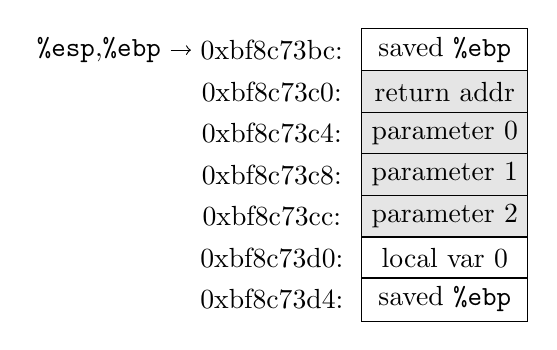
\begin{tikzpicture}
                \tikzset{x=2.5em, y=1.5em}
                \tikzstyle{mem}=[rectangle, draw, minimum width=6em, minimum height=1.5em]
                \tikzstyle{frame}=[mem, fill=black!10]

                \draw (0.0, 6.0)    node        (ep)    {\esp,\ebp};

                \draw (2.5, 6.0)    node        (a6)    {0xbf8c73bc:};
                \draw (2.5, 5.0)    node        (a5)    {0xbf8c73c0:};
                \draw (2.5, 4.0)    node        (a4)    {0xbf8c73c4:};
                \draw (2.5, 3.0)    node        (a3)    {0xbf8c73c8:};
                \draw (2.5, 2.0)    node        (a2)    {0xbf8c73cc:};
                \draw (2.5, 1.0)    node        (a1)    {0xbf8c73d0:};
                \draw (2.5, 0.0)    node        (a0)    {0xbf8c73d4:};

                \draw (5.0, 6.0)    node[mem]   (sebp)  {saved \ebp};
                \draw (5.0, 5.0)    node[frame] (raddr) {return addr};
                \draw (5.0, 4.0)    node[frame] (p0)    {parameter 0};
                \draw (5.0, 3.0)    node[frame] (p1)    {parameter 1};
                \draw (5.0, 2.0)    node[frame] (p2)    {parameter 2};
                \draw (5.0, 1.0)    node[mem]   (s1)    {local var 0};
                \draw (5.0, 0.0)    node[mem]   (s0)    {saved \ebp};

                \draw [->]          (ep) -- (a6);
            \end{tikzpicture}
        \end{center}
    }

    \frame{
        \frametitle{Function calls -- stack diagram}
        \begin{center}
            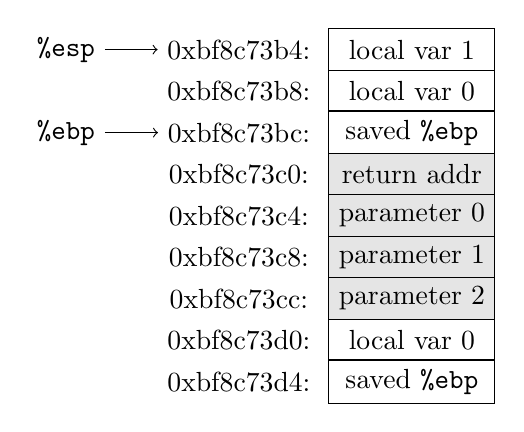
\begin{tikzpicture}
                \tikzset{x=2.5em, y=1.5em}
                \tikzstyle{mem}=[rectangle, draw, minimum width=6em, minimum height=1.5em]
                \tikzstyle{frame}=[mem, fill=black!10]

                \draw (0.0, 8.0)    node        (esp)   {\esp};
                \draw (0.0, 6.0)    node        (ebp)   {\ebp};

                \draw (2.5, 8.0)    node        (a8)    {0xbf8c73b4:};
                \draw (2.5, 7.0)    node        (a7)    {0xbf8c73b8:};
                \draw (2.5, 6.0)    node        (a6)    {0xbf8c73bc:};
                \draw (2.5, 5.0)    node        (a5)    {0xbf8c73c0:};
                \draw (2.5, 4.0)    node        (a4)    {0xbf8c73c4:};
                \draw (2.5, 3.0)    node        (a3)    {0xbf8c73c8:};
                \draw (2.5, 2.0)    node        (a2)    {0xbf8c73cc:};
                \draw (2.5, 1.0)    node        (a1)    {0xbf8c73d0:};
                \draw (2.5, 0.0)    node        (a0)    {0xbf8c73d4:};

                \draw (5.0, 8.0)    node[mem]   (v1)    {local var 1};
                \draw (5.0, 7.0)    node[mem]   (v0)    {local var 0};
                \draw (5.0, 6.0)    node[mem]   (sebp)  {saved \ebp};
                \draw (5.0, 5.0)    node[frame] (raddr) {return addr};
                \draw (5.0, 4.0)    node[frame] (p0)    {parameter 0};
                \draw (5.0, 3.0)    node[frame] (p1)    {parameter 1};
                \draw (5.0, 2.0)    node[frame] (p2)    {parameter 2};
                \draw (5.0, 1.0)    node[mem]   (s1)    {local var 0};
                \draw (5.0, 0.0)    node[mem]   (s0)    {saved \ebp};

                \draw [->]          (esp) -- (a8);
                \draw [->]          (ebp) -- (a6);
            \end{tikzpicture}
        \end{center}
    }


\subsection{Stack buffer overflow}
    \frame{
        \frametitle{Before...}
        \begin{center}
            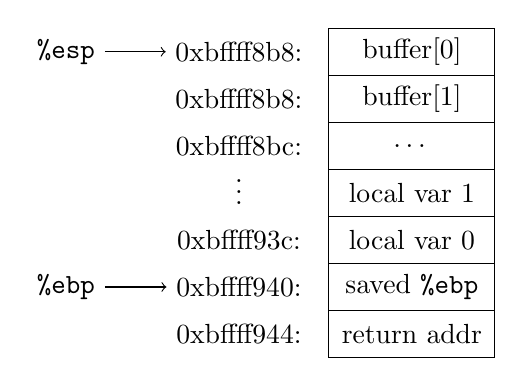
\begin{tikzpicture}
                \tikzset{x=2.5em, y=1.7em}
                \tikzstyle{mem}=[rectangle, draw, minimum width=6em, minimum height=1.7em]

                \draw (0.0, 6.0)    node        (esp)   {\esp};
                \draw (0.0, 1.0)    node        (ebp)   {\ebp};

                \draw (2.5, 6.0)    node        (a6)    {0xbffff8b8:};
                \draw (2.5, 5.0)    node        (a5)    {0xbffff8b8:};
                \draw (2.5, 4.0)    node        (a4)    {0xbffff8bc:};
                \draw (2.5, 3.2)    node        (a3)    {$\vdots$};
                \draw (2.5, 2.0)    node        (a2)    {0xbffff93c:};
                \draw (2.5, 1.0)    node        (a1)    {0xbffff940:};
                \draw (2.5, 0.0)    node        (a0)    {0xbffff944:};

                \draw (5.0, 6.0)    node[mem]   (b1)    {buffer[0]};
                \draw (5.0, 5.0)    node[mem]   (b1)    {buffer[1]};
                \draw (5.0, 4.0)    node[mem]   (b2)    {\dots};
                \draw (5.0, 3.0)    node[mem]   (v1)    {local var 1};
                \draw (5.0, 2.0)    node[mem]   (v0)    {local var 0};
                \draw (5.0, 1.0)    node[mem]   (sebp)  {saved \ebp};
                \draw (5.0, 0.0)    node[mem]   (raddr) {return addr};

                \draw [->]          (esp) -- (a6);
                \draw [->]          (ebp) -- (a1);
            \end{tikzpicture}
        \end{center}
    }

    \frame{
        \frametitle{Meanwhile...}
        \begin{center}
            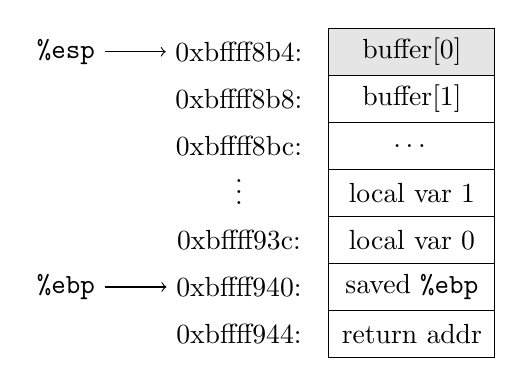
\begin{tikzpicture}
                \tikzset{x=2.5em, y=1.7em}
                \tikzstyle{mem}=[rectangle, draw, minimum width=6em, minimum height=1.7em]
                \tikzstyle{frame}=[mem, fill=black!10]

                \draw (0.0, 6.0)    node        (esp)   {\esp};
                \draw (0.0, 1.0)    node        (ebp)   {\ebp};

                \draw (2.5, 6.0)    node        (a6)    {0xbffff8b4:};
                \draw (2.5, 5.0)    node        (a5)    {0xbffff8b8:};
                \draw (2.5, 4.0)    node        (a4)    {0xbffff8bc:};
                \draw (2.5, 3.2)    node        (a3)    {$\vdots$};
                \draw (2.5, 2.0)    node        (a2)    {0xbffff93c:};
                \draw (2.5, 1.0)    node        (a1)    {0xbffff940:};
                \draw (2.5, 0.0)    node        (a0)    {0xbffff944:};

                \draw (5.0, 6.0)    node[frame] (b0)    {buffer[0]};
                \draw (5.0, 5.0)    node[mem]   (b1)    {buffer[1]};
                \draw (5.0, 4.0)    node[mem]   (b2)    {\dots};
                \draw (5.0, 3.0)    node[mem]   (v1)    {local var 1};
                \draw (5.0, 2.0)    node[mem]   (v0)    {local var 0};
                \draw (5.0, 1.0)    node[mem]   (sebp)  {saved \ebp};
                \draw (5.0, 0.0)    node[mem]   (raddr) {return addr};

                \draw [->]          (esp) -- (a6);
                \draw [->]          (ebp) -- (a1);
            \end{tikzpicture}
        \end{center}
    }

    \frame{
        \frametitle{Meanwhile...}
        \begin{center}
            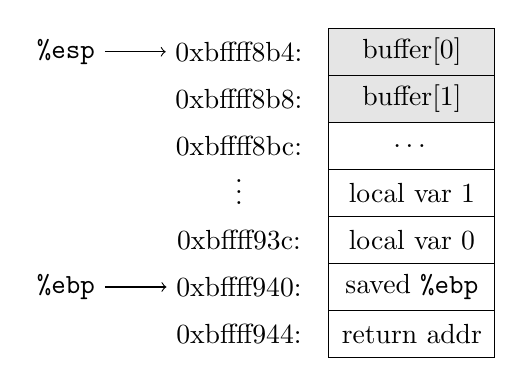
\begin{tikzpicture}
                \tikzset{x=2.5em, y=1.7em}
                \tikzstyle{mem}=[rectangle, draw, minimum width=6em, minimum height=1.7em]
                \tikzstyle{frame}=[mem, fill=black!10]

                \draw (0.0, 6.0)    node        (esp)   {\esp};
                \draw (0.0, 1.0)    node        (ebp)   {\ebp};

                \draw (2.5, 6.0)    node        (a6)    {0xbffff8b4:};
                \draw (2.5, 5.0)    node        (a5)    {0xbffff8b8:};
                \draw (2.5, 4.0)    node        (a4)    {0xbffff8bc:};
                \draw (2.5, 3.2)    node        (a3)    {$\vdots$};
                \draw (2.5, 2.0)    node        (a2)    {0xbffff93c:};
                \draw (2.5, 1.0)    node        (a1)    {0xbffff940:};
                \draw (2.5, 0.0)    node        (a0)    {0xbffff944:};

                \draw (5.0, 6.0)    node[frame] (b0)    {buffer[0]};
                \draw (5.0, 5.0)    node[frame] (b1)    {buffer[1]};
                \draw (5.0, 4.0)    node[mem]   (b2)    {\dots};
                \draw (5.0, 3.0)    node[mem]   (v1)    {local var 1};
                \draw (5.0, 2.0)    node[mem]   (v0)    {local var 0};
                \draw (5.0, 1.0)    node[mem]   (sebp)  {saved \ebp};
                \draw (5.0, 0.0)    node[mem]   (raddr) {return addr};

                \draw [->]          (esp) -- (a6);
                \draw [->]          (ebp) -- (a1);
            \end{tikzpicture}
        \end{center}
    }

    \frame{
        \frametitle{Meanwhile...}
        \begin{center}
            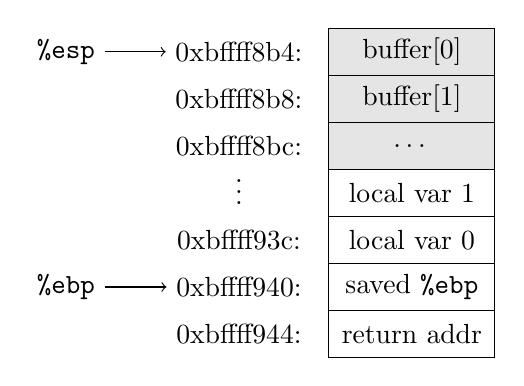
\begin{tikzpicture}
                \tikzset{x=2.5em, y=1.7em}
                \tikzstyle{mem}=[rectangle, draw, minimum width=6em, minimum height=1.7em]
                \tikzstyle{frame}=[mem, fill=black!10]

                \draw (0.0, 6.0)    node        (esp)   {\esp};
                \draw (0.0, 1.0)    node        (ebp)   {\ebp};

                \draw (2.5, 6.0)    node        (a6)    {0xbffff8b4:};
                \draw (2.5, 5.0)    node        (a5)    {0xbffff8b8:};
                \draw (2.5, 4.0)    node        (a4)    {0xbffff8bc:};
                \draw (2.5, 3.2)    node        (a3)    {$\vdots$};
                \draw (2.5, 2.0)    node        (a2)    {0xbffff93c:};
                \draw (2.5, 1.0)    node        (a1)    {0xbffff940:};
                \draw (2.5, 0.0)    node        (a0)    {0xbffff944:};

                \draw (5.0, 6.0)    node[frame] (b0)    {buffer[0]};
                \draw (5.0, 5.0)    node[frame] (b1)    {buffer[1]};
                \draw (5.0, 4.0)    node[frame] (b2)    {\dots};
                \draw (5.0, 3.0)    node[mem]   (v1)    {local var 1};
                \draw (5.0, 2.0)    node[mem]   (v0)    {local var 0};
                \draw (5.0, 1.0)    node[mem]   (sebp)  {saved \ebp};
                \draw (5.0, 0.0)    node[mem]   (raddr) {return addr};

                \draw [->]          (esp) -- (a6);
                \draw [->]          (ebp) -- (a1);
            \end{tikzpicture}
        \end{center}
    }

    \frame{
        \frametitle{Meanwhile...}
        \begin{center}
            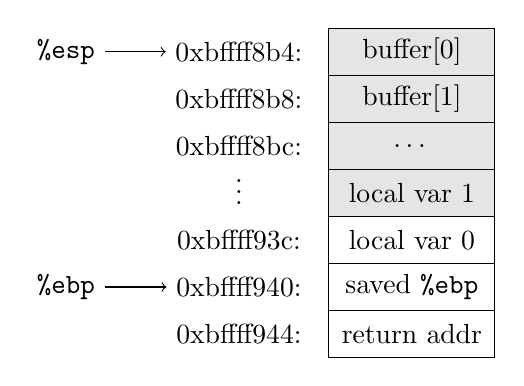
\begin{tikzpicture}
                \tikzset{x=2.5em, y=1.7em}
                \tikzstyle{mem}=[rectangle, draw, minimum width=6em, minimum height=1.7em]
                \tikzstyle{frame}=[mem, fill=black!10]

                \draw (0.0, 6.0)    node        (esp)   {\esp};
                \draw (0.0, 1.0)    node        (ebp)   {\ebp};

                \draw (2.5, 6.0)    node        (a6)    {0xbffff8b4:};
                \draw (2.5, 5.0)    node        (a5)    {0xbffff8b8:};
                \draw (2.5, 4.0)    node        (a4)    {0xbffff8bc:};
                \draw (2.5, 3.2)    node        (a3)    {$\vdots$};
                \draw (2.5, 2.0)    node        (a2)    {0xbffff93c:};
                \draw (2.5, 1.0)    node        (a1)    {0xbffff940:};
                \draw (2.5, 0.0)    node        (a0)    {0xbffff944:};

                \draw (5.0, 6.0)    node[frame] (b0)    {buffer[0]};
                \draw (5.0, 5.0)    node[frame] (b1)    {buffer[1]};
                \draw (5.0, 4.0)    node[frame] (b2)    {\dots};
                \draw (5.0, 3.0)    node[frame] (v1)    {local var 1};
                \draw (5.0, 2.0)    node[mem]   (v0)    {local var 0};
                \draw (5.0, 1.0)    node[mem]   (sebp)  {saved \ebp};
                \draw (5.0, 0.0)    node[mem]   (raddr) {return addr};

                \draw [->]          (esp) -- (a6);
                \draw [->]          (ebp) -- (a1);
            \end{tikzpicture}
        \end{center}
    }

    \frame{
        \frametitle{Boom!}
        \begin{center}
            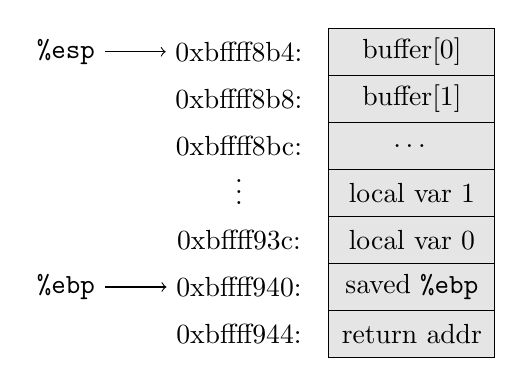
\begin{tikzpicture}
                \tikzset{x=2.5em, y=1.7em}
                \tikzstyle{mem}=[rectangle, draw, minimum width=6em, minimum height=1.7em]
                \tikzstyle{frame}=[mem, fill=black!10]

                \draw (0.0, 6.0)    node        (esp)   {\esp};
                \draw (0.0, 1.0)    node        (ebp)   {\ebp};

                \draw (2.5, 6.0)    node        (a6)    {0xbffff8b4:};
                \draw (2.5, 5.0)    node        (a5)    {0xbffff8b8:};
                \draw (2.5, 4.0)    node        (a4)    {0xbffff8bc:};
                \draw (2.5, 3.2)    node        (a3)    {$\vdots$};
                \draw (2.5, 2.0)    node        (a2)    {0xbffff93c:};
                \draw (2.5, 1.0)    node        (a1)    {0xbffff940:};
                \draw (2.5, 0.0)    node        (a0)    {0xbffff944:};

                \draw (5.0, 6.0)    node[frame] (b0)    {buffer[0]};
                \draw (5.0, 5.0)    node[frame] (b1)    {buffer[1]};
                \draw (5.0, 4.0)    node[frame] (b2)    {\dots};
                \draw (5.0, 3.0)    node[frame] (v1)    {local var 1};
                \draw (5.0, 2.0)    node[frame] (v0)    {local var 0};
                \draw (5.0, 1.0)    node[frame] (sebp)  {saved \ebp};
                \draw (5.0, 0.0)    node[frame] (raddr) {return addr};

                \draw [->]          (esp) -- (a6);
                \draw [->]          (ebp) -- (a1);
            \end{tikzpicture}
        \end{center}
    }



\subsection{Gadgets}
    \frame{
        \frametitle{What is a gadget?}
        \begin{itemize}
            \item attacker searches for short instruction sequences that perform small tasks and end with \ret \\
                  \lto\ for example \pop ing some values into registers
            \item gadget: combination of one or more short instruction sequence addresses and the values that they \pop\ off the stack
            \item payload: chain of gadgets
        \end{itemize}
    }

    \frame{
        \frametitle{A very simple gadget}
        \begin{center}
            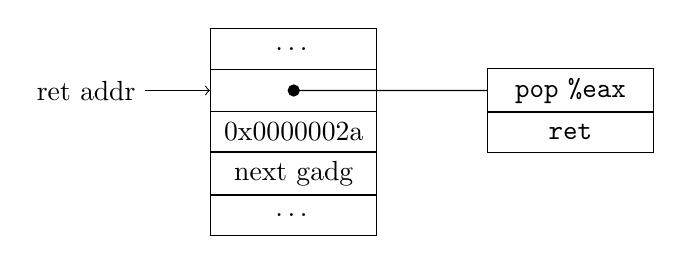
\begin{tikzpicture}
                \tikzset{x=2.5em, y=1.5em, radius=2pt, fill=black}
                \tikzstyle{mem}=[rectangle, draw, minimum width=6em, minimum height=1.5em]

                % annotations
                \draw (0.0, 3.0)    node        (ret)   {ret addr};

                % stack
                \draw (3.0, 4.0)    node[mem]   (s4)    {\dots};
                \draw (3.0, 3.0)    node[mem]   (s3)    {};
                \draw (3.0, 2.0)    node[mem]   (s2)    {0x0000002a};
                \draw (3.0, 1.0)    node[mem]   (s1)    {next gadg};
                \draw (3.0, 0.0)    node[mem]   (s0)    {\dots};

                % first fake stack frame
                \draw (7.0, 3.0)    node[mem]   (i0)    {\pop\ \eax};
                \draw (7.0, 2.0)    node[mem]   (i1)    {\ret};

                % annotation arrows
                \draw [->]          (ret) -- (s3);

                % memory pointer arrows
                \filldraw           (s3.center)  circle -- (i0.west);
            \end{tikzpicture}
        \end{center}
    }

    \section{Demonstration}
\subsection{ROPgadget -- a ROP compiler}
    \frame{
        \frametitle{\ropgadget}
        \begin{itemize}
            \item finds and lists gadgets that are available in a specified binary
            \item constructs \shellcode, a \payload\ that opens a network socket or user-specified opcodes
            \item prints out python commands that can be embedded in a \payload\ generation script
            \item searches and prints out addresses of instructions/opcodes and strings in a binary
        \end{itemize}
    }



\subsection{Stupid vulnerable program}
    \frame{
        \frametitle{log.h}
        \scriptsize
        \inputminted[linenos,tabsize=4]{c}{demo/log.h}
    }

    \frame{
        \frametitle{log.c}
        \scriptsize
        \inputminted[linenos,tabsize=4]{c}{demo/log.c}
    }

    \frame{
        \frametitle{io.c}
        \scriptsize
        \inputminted[linenos,tabsize=4]{c}{demo/io.c}
    }

    \frame{
        \frametitle{util.c}
        \scriptsize
        \inputminted[linenos,tabsize=4]{c}{demo/util.c}
    }



\subsection{Showtime!}
    \frame{
        \frametitle{The fun part...}
        \begin{center}
            \Huge
            Showtime!
        \end{center}
    }

    \section{Countermeasures}
\subsection{Address space layout randomization}



\subsection{Stack canaries}

    \section{Conclusion}

\frame{
    \begin{itemize}
        \item long evolution from direct code injection to ROP
        \item applicable to many popular architectures
        \item quite complex technique
        \item relatively recent $\leadsto$ few effective countermeasures
        \item frameworks for automation of \payload\ generation
        \item $\leadsto$ serious threat!
        \item But: It's fun! \Smiley
    \end{itemize}
}


    \section{}
    \frame{
        \begin{center}
        {\Large\bfseries Thanks for your attention.} \\[5mm]
        Questions?
        \end{center}
    }
\end{document}

